\documentclass[useAMS,usenatbib]{mn2e}
\pdfminorversion=4

% The following is needed to fix the margins if using Letter-size paper
% REMOVE if your LaTeX uses A4 paper by default
\addtolength\topmargin{-1.8cm}
\usepackage{newtxtext}
\usepackage[varg]{newtxmath}

\usepackage{graphicx}
\usepackage{booktabs}
\usepackage{siunitx}
\bibliographystyle{mn2e}
\usepackage{astrojournals}
\usepackage{fixltx2e}

\begin{document}

\newcounter{ion}
\newcommand\fakesc[1]{\protect\scalebox{1.0}[0.8]{#1}}
\newcommand\ION[2]{\ensuremath{\mathrm{#1\,\fakesc{#2}}}}
\newcommand\ion[2]{\setcounter{ion}{#2}\ION{#1}{\Roman{ion}}}
\newcommand\hii{\ion{H}{2}}
\newcommand\oi{[\ion{O}{1}]}
\newcommand\oiii{[\ion{O}{3}]}
\newcommand\nii{[\ion{N}{2}]}
\newcommand\sii{[\ion{S}{2}]}
\newcommand\siii{[\ion{S}{3}]}
\newcommand\ha{\ensuremath{\mathrm{H\alpha}}}
\newcommand\kms{\ensuremath{\mathrm{km\ s^{-1}}}}
\newcommand\los{\ensuremath{_{\mathrm{los}}}}
\newcommand\pos{\ensuremath{_{\mathrm{pos}}}}
\newcommand\obs{\ensuremath{_{\mathrm{obs}}}}
\newcommand\ins{\ensuremath{_{\mathrm{ins}}}}
\newcommand\rms{\ensuremath{_{\mathrm{rms}}}}
\newcommand\FS{\ensuremath{_{\mathrm{fs}}}}
\newcommand\therm{\ensuremath{_{\mathrm{therm}}}}

\newcommand\Efrac{\ensuremath{_{\scriptscriptstyle E/E_0}}}
\newcommand\denfrac{\ensuremath{_{\scriptscriptstyle \rho/\rho_0}}}
\newcommand\lnSfrac{\ensuremath{_{\scriptscriptstyle \ln S/S_0}}}
\newcommand\Sfrac{\ensuremath{_{\scriptscriptstyle S/S_0}}}


\addtocounter{section}{5}

\section{Summary and Speculation}
\label{sec:summary-conclusions}

We have used statistical analysis of high-resolution spectroscopic
observations of optical emission lines in the central
\(0.4 \times 0.6\)~pc of the Orion Nebula in order to characterize the
turbulence in the ionized gas. The analysis has been guided and
informed by radiation hydrodynamic simulations of \hii{} region
evolution. The techniques that we have applied are:
\begin{enumerate}
\item Second order structure function of velocity centroids, which
  gives the variation as a function of plane-of-sky separation of the
  average velocity integrated along the line of sight.
\item Velocity channel analysis (VCA), which compares the spatial
  power spectrum slope of velocity-resolved and velocity-integrated
  emission profiles of the same line.
\item Line width analysis, which is sensitive to velocity fluctuations
  along the line of sight
\item Probability density function (PDF) of the surface brightness in
  different lines
\end{enumerate}
Our principal empirical findings are as follows:
\begin{enumerate}
\item The VCA technique is the most reliable means of determining the
  spectrum of velocity fluctuations in the ionized gas, and we find
  consistent evidence from both low and high ionization lines for a
  Kolmogorov-type spectrum (\(\delta u \sim l^{1/3}\)) for length
  scales, \(l\), between \(0.05\)~pc (\(\approx 22''\)) and \(0.02\)~pc
  (\(\approx 8''\)).  Unfortunately, VCA can not be applied if the
  thermal or instrumental line width is larger than the velocity
  differences of interest, which rules out its application to the
  \ha{} line and to scales smaller than \(0.02\)~pc. 
\item The structure functions show systematic trends with degree of
  ionization.  Higher ionization lines tend to show larger
  autocorrelation scales, larger total plane-of-sky velocity
  dispersions, and steeper slopes than lower ionization lines.  The
  changes in slopes are difficult to interpret because of the
  influence of projection smearing and sensitivity to details of the
  observational methodology.
% Correlation length from struc func
\item The characteristic length of \(0.05\)~pc is special in at least
  two ways, corresponding to both the autocorrelation scale of
  velocity differences for low-ionization lines and also a break in
  the power spectrum of surface brightness fluctuations in all lines.
  We suggest that this is the dominant scale for density fluctuations
  in the nebula and is also the main driving scale of the
  turbulence. A further break in the surface brightness power spectra
  occurs at the smaller scale of \(0.02\)~pc (\(\approx 8''\)), but
  there is no obvious feature in the structure functions at this
  scale.
% Velocity dispersion
\item There are three lines of evidence suggesting that the velocity
  fluctuations are not homogeneous on the largest scales, but rather
  that the turbulent conditions themselves vary, both across the sky and
  along the line of sight, on scales larger than the velocity
  autocorrelation length of \(0.05\)--\(0.15\)~pc:
  \begin{enumerate}
  \item The structure function slope of the \nii{} line is
    significantly steeper in the southern half of our observed field
    than in the northern half
  \item The plane-of-sky velocity dispersion increases with increasing
    ionization, implying an increasing amplitude of fluctuations
    towards the interior of the nebula
  \item The line-of-sight non-thermal velocity dispersion (after
    removing the confounding effect of dust scattering) is typically
    twice as large (\(\approx 6~\kms\)) as the plane-of-sky velocity
    dispersion (\(\approx 6~\kms\)).  In order to explain this ratio
    in terms of a homogeneous turbulent layer, the line-of-sight depth
    of the layer would need to be at least 10 times the velocity
    autocorrelation length, which is unrealistically large.  Instead,
    the result is more naturally explained by large-scale velocity
    gradients (such as radial expansion), combined with emissivity
    fluctuations along the line of sight.
  \end{enumerate}
% PDF of surface brightness
\item The PDF of surface brightness fluctuations is approximately
  log-normal with a fractional width of \(0.4\)--\(0.5\) in all lines.
  The amplitude of these fluctuations is marginally consistent with
  their having being wholly caused by the observed velocity
  fluctuations, so long as the velocity field is irrotational at the
  driving scale. 
% Turbulent vs ordered velocities
\item The ordered component of the velocity dispersion can be
  estimated to be \(\approx 4.5~\kms\), which implies that the
  turbulent component is of roughly similar magnitude so that their
  quadrature sum gives the observed total dispersion of \(6~\kms\). 
\end{enumerate}

\begin{figure}
  \centering
  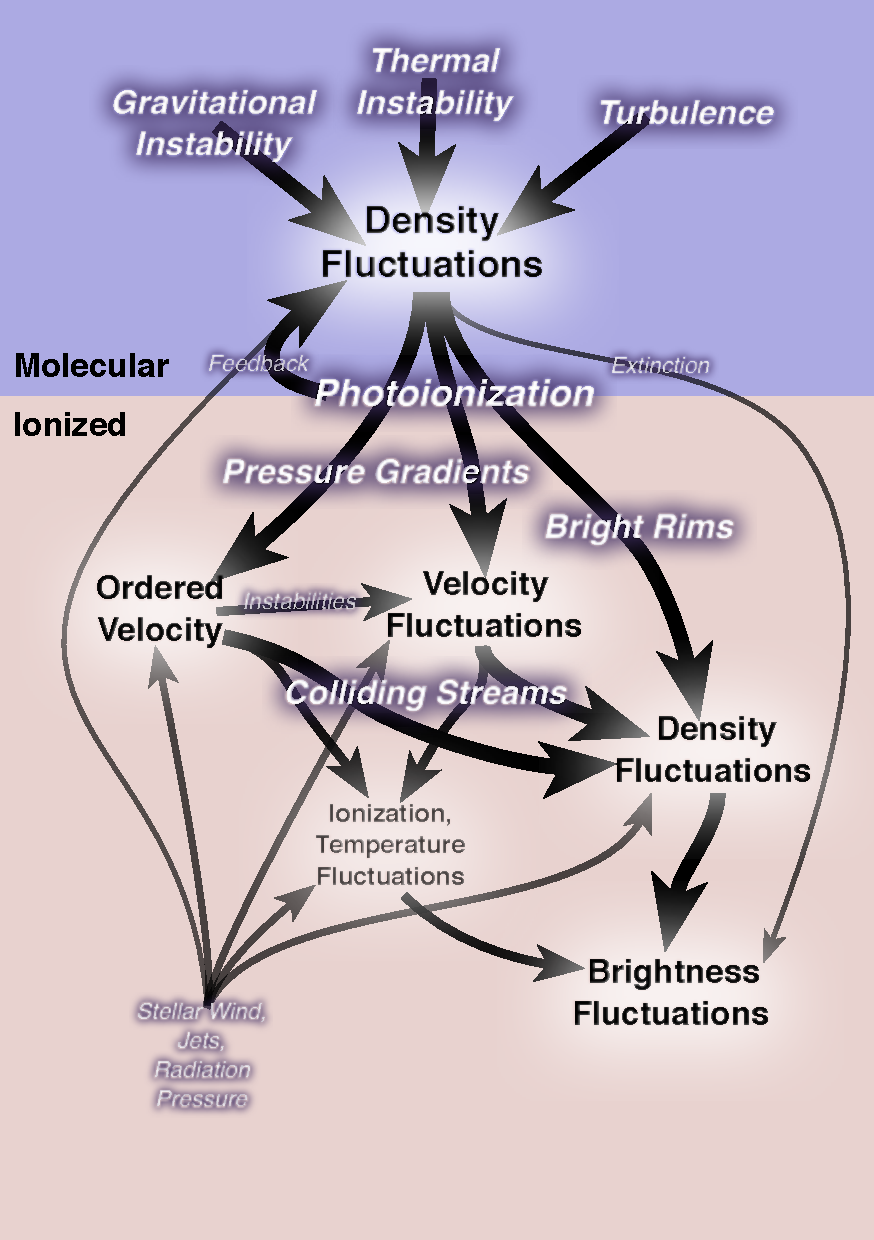
\includegraphics[width=\linewidth]{causality-flow}
  \caption{Causal relationships (arrows) between different types of
    fluctuations (black text) in molecular clouds (above) and \hii{}
    regions (below) via different physical processes (white text).
    Line thickness and text size is proportional to the relative
    importance of each process in the Orion Nebula.}
  \label{fig:causality-flow}
\end{figure}


Finally, we offer a speculative account of the complex web of physical
processes that give rise to to the velocity and brightness
fluctuations that we observe in the Orion Nebula.  This is illustrated
in Figure~\ref{fig:causality-flow}, where the most important causal
links are shown by thick arrows and secondary processes by thin
arrows.  

The principal origin of all structure in the \hii{} region is
the highly filamentary and clumpy density structure in the molecular
cloud from which it is emerging, which in turn has its origin in some
combination of thermal and gravitational instability and supersonic
turbulence \citep{Padoan:2002a, Ballesteros:2011a}.  In the molecular
gas, thermal pressure is negligible compared with magnetic pressure,
turbulent ram pressure, and the gravitational potential.  However, the
large temperature increase that accompanies photoionization means that
thermal pressure dominates in the \hii{} region, so that density
gradients are converted into pressure gradients that can accelerate
the gas.  The fractal nature of the molecular density means that gas
acceleration occurs on multiple scales, from the global outward radial
expansion of the \hii{} region (which in Orion is a highly one-sided
champagne flow) down to photoevaporation flows from individual
globules.   One piece of evidence for a direct connection between
molecular density fluctuations and ionized velocity fluctuations is
that \citet{Kainulainen:2016a} find correlation lengths of order \(0.08\)~pc
for the separations of molecular cores along the ridge that lies
behind the Orion Nebula, which is similar to the correlation lengths
we find for the velocity fluctuations in the nebula. 

Ionized density fluctuations can arise directly from the molecular
density fluctuations, such as the bright rims at the edges of
photoionized globules \citep{Henney:2009a}, and this is most important
in the lower ionization zones near the ionization front where the
\sii{} and \nii{} emission is strong.  In the more highly ionized
interior of the nebula, it is collisions between opposing velocity
streams that produce the ionized density fluctuations, but these
fluctuations are less extreme than those seen in molecular gas because
the turbulence is subsonic.

The ionized density fluctuations are the primary determinant of the
emission line surface brightness fluctuations (\S~4.5), although
ionization and temperature structure can make a contribution for
particular lines and there is also a direct contribution from
foreground molecular density fluctuations via dust extinction
\citep{ODell:2000a}.

Finally, a variety of other processes, such as O~star winds, radiation
pressure, and bipolar jets from young stars can play a secondary role
in stirring up gas motions.  In the case of the Orion Nebula, evidence
for the influence of stellar wind interactions is restricted to the
central \(0.05\)~pc \citep{Garcia-Arredondo:2001a} and the low-density
western outskirts \citep{Gudel:2008a}, and they seem to have little
influence on the bulk of the nebular gas.  Stellar wind effects are
more important in older and more massive regions that contain LBV and
Wolf-Rayet stars (e.g., \citealp{Smith:2007a}).  Similarly, radiation
pressure, although unimportant in Orion, becomes much more important
in higher luminosity regions \citep{Krumholz:2009a}.  Herbig-Haro jets
and bowshocks dominate the far wings (\(\delta u \sim 50~\kms\)) of
the velocity distribution in Orion \citep{Henney:2007b}, but the total
kinetic energy of these high velocity flows is relatively low, so that
the effect on the global velocity statistics is minor.


\bibliography{BibdeskLibrary-slavoj}

\end{document}
%%% Local Variables:
%%% mode: latex
%%% TeX-master: t
%%% End:
